\section{Propuesta de Rediseño}

La propuesta de rediseño se construye a partir de los problemas prioritarios identificados en WebSIS y de las necesidades detectadas en estudiantes ingresantes y avanzados. Su objetivo no es agregar funciones nuevas, sino reorganizar las existentes para que las tareas criticas puedan completarse con menor carga cognitiva, mayor claridad de estado y mejor compatibilidad movil.

\subsection{Funcionalidades intervenidas}

El rediseño considera las secciones criticas observadas en el sistema actual y define una intervencion especifica para cada una:

\begin{itemize}
  \item \textbf{Pantalla de bienvenida:} se elimina la pantalla informativa inicial que obligaba a entrar manualmente al acceso de estudiantes. El sistema pasa directamente al inicio de sesion, reduciendo un paso sin valor operativo.
  \item \textbf{Inicio de sesion de estudiante:} se reemplaza el formulario antiguo basado en dia, mes y año separados por una entrada directa de fecha con formato visible. Tambien se elimina el codigo visual tipo CAPTCHA, considerado anticuado y costoso para el usuario.
  \item \textbf{Panel del estudiante:} se elimina informacion irrelevante y se conservan solamente accesos de uso frecuente, estado academico y acciones prioritarias.
  \item \textbf{Informacion general:} los datos personales dejan de ocupar un bloque lateral permanente y se trasladan al menu de perfil, donde pueden consultarse cuando el estudiante los necesita.
  \item \textbf{Pago de matricula:} se agrega un estado visible de matricula pagada y un acceso explicito a \textit{Pagar matricula}. Si el pago ya fue confirmado, el boton permanece visible pero deshabilitado para evitar pagos duplicados.
  \item \textbf{Kardex:} se reorganiza la visualizacion de notas, se reducen columnas innecesarias y se diferencia entre materias cerradas y materias en curso.
  \item \textbf{Inscripcion a materias:} se separa la validacion de codigos del proceso de tomar materias, se agrega limite visible, seleccion de grupo, modalidad y resumen final.
  \item \textbf{Obtencion y validacion de codigos:} los codigos se validan antes del periodo de inscripcion para habilitar la cuenta y evitar repetir el paso durante el momento critico.
  \item \textbf{Horario de clases:} se muestra directamente el horario vigente del estudiante, sin pedir gestiones o periodos irrelevantes.
  \item \textbf{Cambio de contraseña:} se traslada al menu de perfil como accion de seguridad, evitando que aparezca mezclado con tareas academicas principales.
\end{itemize}

\subsection{Estructura del contenido}

La estructura del contenido fue redefinida desde la logica de tareas del estudiante y no desde la organizacion tecnica interna del sistema. Se priorizan las acciones de mayor frecuencia y criticidad:

\begin{itemize}
  \item \textbf{Acceso al sistema:} inicio de sesion directo, sin pantalla de bienvenida previa ni controles de seguridad obsoletos.
  \item \textbf{Inicio:} panel principal con accesos directos a las tareas mas frecuentes y estado general de la gestion academica actual.
  \item \textbf{Matricula:} verificacion del pago, comprobante, entidad y acceso a pago cuando corresponda.
  \item \textbf{Inscripcion:} flujo principal para seleccionar materias, grupos y modalidad de cursado dentro de un mismo contexto.
  \item \textbf{Validacion de codigos:} paso previo y separado del modulo de inscripcion, utilizado para habilitar la cuenta antes del periodo critico.
  \item \textbf{Estado de inscripcion:} resumen posterior al registro de materias con confirmacion clara del resultado de la accion.
  \item \textbf{Horario de clases:} visualizacion directa del horario vigente sin obligar al estudiante a atravesar filtros irrelevantes.
  \item \textbf{Kardex:} historial academico con diferenciacion entre materias finalizadas y materias aun en curso.
  \item \textbf{Perfil y seguridad:} datos generales del estudiante y cambio de contraseña dentro del menu de usuario.
  \item \textbf{Soporte contextual:} mensajes, aclaraciones y estados integrados dentro de cada pantalla en lugar de depender de ayuda externa.
\end{itemize}

Esta estructura responde directamente a las necesidades N1, N2, N5, N6 y N8 detectadas en la investigacion.

\subsection{Mapa del sistema}

El sistema rediseñado se organiza a partir de una navegacion corta y reconocible:

\begin{center}
\resizebox{\textwidth}{!}{%
\begin{tikzpicture}[
  x=1cm, y=1cm,
  box/.style={draw, rounded corners=2pt, align=center, text width=3.2cm, minimum height=1cm, inner sep=3pt, font=\small},
  ruta/.style={},
  prereq/.style={-Latex, densely dashed, color=black!55},
  flow/.style={-Latex}
]
  % Acceso (centrado en x=0)
  \node[box] (login)  at (0, 9)  {\textbf{Inicio de sesion}\\[1pt]{\scriptsize\ttfamily\color{black!55} /}};
  \node[box] (inicio) at (0, 6.6) {\textbf{Panel del estudiante}\\[1pt]{\scriptsize\ttfamily\color{black!55} /panel}};

  % Fila intermedia: 4 accesos del panel, separados 4cm en x
  \node[box] (matricula) at (-6, 3.6) {Matricula\\[1pt]{\scriptsize\ttfamily\color{black!55} /panel/matricula}};
  \node[box] (codigo)    at (-2, 3.6) {Codigo de inscripcion\\[1pt]{\scriptsize\ttfamily\color{black!55} /panel/codigo}};
  \node[box] (kardex)    at ( 2, 3.6) {Kardex\\[1pt]{\scriptsize\ttfamily\color{black!55} /panel/kardex}};
  \node[box] (horario)   at ( 6, 3.6) {Horario de clases\\[1pt]{\scriptsize\ttfamily\color{black!55} /panel/horario}};

  % Flujo central de inscripcion (centrado)
  \node[box] (inscripcion) at (0, 1)   {\textbf{Inscripcion a materias}\\[1pt]{\scriptsize\ttfamily\color{black!55} /panel/inscripcion}};
  \node[box] (estado)      at (0, -1.6) {Estado de inscripcion\\[1pt]{\scriptsize\ttfamily\color{black!55} /panel/estado}};

  % Perfil (solo desde menu de usuario), a la derecha del panel
  \node[box] (seguridad) at (6, 6.6) {Perfil y seguridad\\[1pt]{\scriptsize\ttfamily\color{black!55} /panel/seguridad}};

  % Acceso
  \draw[flow] (login) -- (inicio);

  % El panel es punto de entrada a todas las secciones
  \draw[flow] (inicio) -- (matricula);
  \draw[flow] (inicio) -- (codigo);
  \draw[flow] (inicio) -- (kardex);
  \draw[flow] (inicio) -- (horario);
  \draw[flow] (inicio) -- (inscripcion);
  % El panel tambien da acceso directo al estado de inscripcion:
  % se rutea por un canal vertical muy a la izquierda (x=-9.2), por fuera de todas las cajas
  \draw[flow] (inicio.west) -- (-9.2, 6.6) -- (-9.2, -1.6) -- (estado.west);
  % Perfil y seguridad se abre desde el menu de usuario, no como tarjeta del panel
  \draw[flow] (inicio) to[bend left=12] node[midway, above, font=\scriptsize\itshape] {menu de usuario} (seguridad);

  % Matricula y codigo son prerequisitos paralelos de la inscripcion (y retornan a ella)
  \draw[prereq] (matricula) -- (inscripcion);
  \draw[prereq] (codigo) -- (inscripcion);

  % La inscripcion deriva al estado: bajada recta por el centro.
  \draw[flow] (inscripcion) -- (estado);
  % El estado vuelve a inscripcion (Modificar): canal vertical propio a la derecha (x=2.6).
  \draw[flow] (estado.east) -- (2.6, -1.6) -- (2.6, 1)
        node[midway, right=1pt, font=\scriptsize\itshape] {modificar} -- (inscripcion.east);
\end{tikzpicture}
}
\end{center}

\begin{center}
\footnotesize
\begin{tabular}{ll}
\tikz{\draw[-Latex] (0,0) -- (0.7,0);} & Navegacion directa desde el panel \\
\tikz{\draw[-Latex, densely dashed, color=black!55] (0,0) -- (0.7,0);} & Prerequisito que habilita la inscripcion y retorna a ella \\
\end{tabular}
\end{center}

La jerarquia evita menus ambiguos y reduce el backtracking. El panel del estudiante (\texttt{/panel}) funciona como punto de entrada unico hacia todas las tareas, sin obligar al estudiante a recordar rutas escondidas. El pago de matricula (\texttt{/panel/matricula}) y la validacion de codigos (\texttt{/panel/codigo}) operan como dos prerequisitos independientes de la inscripcion: el modulo de inscripcion detecta cual falta, enlaza directamente a la pantalla correspondiente y, al completarse, devuelve al estudiante al flujo de inscripcion sin volver a pedir los datos ya validados. El estado de inscripcion (\texttt{/panel/estado}) tambien es accesible directamente desde el panel: una vez seleccionadas las materias, la inscripcion deriva a esta pantalla como confirmacion, y desde ella el estudiante puede volver al modulo de inscripcion mediante la opcion \textit{Modificar inscripcion} para ajustar materias, grupos o modalidad. La seccion de perfil y seguridad (\texttt{/panel/seguridad}) no aparece como tarjeta del panel sino que se abre desde el menu de usuario, junto con los datos personales y los enlaces academicos externos.

\subsection{Flujos de navegacion}

\subsubsection*{Flujo 0: acceso al sistema}

\begin{enumerate}
  \item El estudiante ingresa a WebSIS.
  \item El sistema muestra directamente el formulario de inicio de sesion para estudiantes, sin pantalla de bienvenida intermedia.
  \item El estudiante introduce codigo SIS, contraseña y fecha de nacimiento en formato escrito o mediante calendario.
  \item El sistema valida el acceso sin exigir un codigo visual tipo CAPTCHA.
  \item El estudiante ingresa al panel principal.
\end{enumerate}

\subsubsection*{Flujo 1: habilitacion para inscripcion}

\begin{enumerate}
  \item El estudiante ingresa al panel principal.
  \item Verifica el estado de \textit{Matricula}. Si esta pagada, el sistema muestra comprobante, entidad y fecha de registro.
  \item Si no esta pagada, utiliza el acceso \textit{Pagar matricula}; si ya fue confirmada, el boton queda visible pero deshabilitado para evitar pagos duplicados.
  \item Accede a \textit{Validacion de codigos}.
  \item Ingresa dos codigos de acceso requeridos.
  \item El sistema confirma que la cuenta quedo habilitada para inscripcion.
  \item Durante el horario habilitado, el estudiante pasa directamente a \textit{Inscripcion} sin volver a introducir codigos, salvo caso sospechoso.
\end{enumerate}

\subsubsection*{Flujo 2: inscripcion a materias}

\begin{enumerate}
  \item El estudiante entra a \textit{Inscripcion}.
  \item Visualiza el limite maximo de materias disponible para la gestion.
  \item Revisa la oferta de materias recomendadas para su carrera.
  \item Selecciona grupo y modalidad para cada materia.
  \item El sistema muestra las materias elegidas en un resumen lateral persistente.
  \item El estudiante confirma la accion y accede a \textit{Estado de inscripcion}.
  \item El sistema muestra materia, grupo, modalidad, horario, docente y estado final del registro.
\end{enumerate}

\subsubsection*{Flujo 3: consulta de horario}

\begin{enumerate}
  \item El estudiante accede a \textit{Horario de clases} desde el panel principal.
  \item El sistema muestra directamente la gestion vigente y los grupos ya inscritos.
  \item El horario se presenta por dias y bloques, con aula, docente y tipo de clase.
\end{enumerate}

\subsubsection*{Flujo 4: consulta de Kardex}

\begin{enumerate}
  \item El estudiante accede a \textit{Kardex}.
  \item El sistema muestra primero indicadores resumidos del historial academico.
  \item En la tabla, las materias finalizadas se distinguen de las materias en curso.
  \item Si una materia no tiene nota final, el sistema muestra avance por parciales y evita marcarla como reprobada prematuramente.
\end{enumerate}

\subsubsection*{Flujo 5: cambio de contraseña}

\begin{enumerate}
  \item El estudiante abre el menu de perfil.
  \item Selecciona \textit{Cambiar contraseña}.
  \item Ingresa contraseña actual, nueva contraseña y confirmacion.
  \item El sistema confirma el cambio y recomienda cerrar sesiones activas.
\end{enumerate}

\subsection{Wireframes de baja fidelidad}

Los wireframes de baja fidelidad definen la distribucion espacial de bloques, la jerarquia visual y la secuencia de acciones de cada pantalla antes de cualquier tratamiento de alta fidelidad. Cada esquema representa la posicion relativa de los elementos en la interfaz, no su estilo final.

% ---- Estilos de wireframe (uniformes para toda la subseccion) ----
\newcommand{\wfhead}[1]{%
  \setlength{\fboxsep}{8pt}%
  \colorbox{black!75}{\parbox[c][0.5cm][c]{0.96\linewidth}{\centering\color{white}\footnotesize\bfseries #1}}\\[12pt]%
}
\newcommand{\wfsection}[1]{%
  \par\vspace{4pt}%
  \noindent\textcolor{black!50}{\rule{0.96\linewidth}{0.3pt}}\\[4pt]%
  {\footnotesize\bfseries\color{black!80} #1}\\[8pt]%
}
\newcommand{\wfbox}[2][0.96\linewidth]{%
  \setlength{\fboxsep}{8pt}%
  \fbox{\parbox[c][0.55cm][c]{#1}{\centering\footnotesize\color{black!80} #2}}%
}
\newcommand{\wfboxleft}[2][0.96\linewidth]{%
  \setlength{\fboxsep}{8pt}%
  \fbox{\parbox[c][0.55cm][c]{#1}{\footnotesize\color{black!80} #2}}%
}
\newcommand{\wfprimary}[2][0.96\linewidth]{%
  \setlength{\fboxsep}{10pt}%
  \fcolorbox{black!75}{black!12}{\parbox[c][0.7cm][c]{#1}{\centering\footnotesize\bfseries #2}}%
}
\newcommand{\wfsoft}[2][0.96\linewidth]{%
  \setlength{\fboxsep}{8pt}%
  \fcolorbox{black!25}{black!4}{\parbox[c][0.55cm][c]{#1}{\centering\footnotesize\color{black!75} #2}}%
}
\newcommand{\wfframe}[2]{%
  \setlength{\fboxsep}{14pt}%
  \fcolorbox{black!70}{white}{\begin{minipage}{#1}#2\end{minipage}}%
}

\subsubsection*{Wireframe 0: inicio de sesion}

\begin{figure}[H]
\centering
\resizebox{0.62\textwidth}{!}{%
\wfframe{12cm}{%
\centering
\wfhead{Acceso al sistema}
\wfsoft{Selector de rol: estudiante / docente / postulante}\\[14pt]
\wfsection{Acceso de estudiante}
\wfbox{Codigo SIS}\\[8pt]
\wfbox{Contrase\~na}\\[8pt]
\wfbox{Fecha de nacimiento (formato visible / calendario)}\\[16pt]
\wfprimary[0.5\linewidth]{Ingresar}\\[16pt]
\wfsoft[0.7\linewidth]{Recuperar contrase\~na}\\[12pt]
{\scriptsize\itshape\color{black!55} Sin pantalla de bienvenida previa.\\Sin CAPTCHA visual.}%
}}
\caption{Wireframe de baja fidelidad: pantalla de inicio de sesion.}
\label{fig:wf-login}
\end{figure}

\subsubsection*{Wireframe 1: panel principal}

\begin{figure}[H]
\centering
\resizebox{0.94\textwidth}{!}{%
\wfframe{18cm}{%
\centering
\wfhead{Logo \hfill Perfil \quad | \quad Tema}
\wfsoft{Hola, [Estudiante] -- [Carrera] -- Gestion [A\~no/Periodo]}\\[16pt]
\begin{minipage}[t]{0.60\linewidth}\centering
\setlength{\fboxsep}{12pt}%
\fcolorbox{black!75}{black!12}{\parbox[c][1.6cm][c]{0.94\linewidth}{\centering\bfseries Inscribirse\\[3pt]\scriptsize\mdseries\itshape accion principal}}
\end{minipage}\hfill
\begin{minipage}[t]{0.34\linewidth}\centering
\setlength{\fboxsep}{10pt}%
\fcolorbox{black!30}{black!4}{\parbox[c][1.6cm][c]{0.94\linewidth}{\centering\footnotesize\color{black!75} Matricula: \bfseries pagada\\[3pt]\mdseries\scriptsize comprobante resumido}}
\end{minipage}\\[18pt]
\begin{minipage}{0.46\linewidth}\centering\wfbox[0.94\linewidth]{Pagar matricula}\end{minipage}\hfill
\begin{minipage}{0.46\linewidth}\centering\wfbox[0.94\linewidth]{Validar codigos}\end{minipage}\\[16pt]
\wfsection{Accesos directos}
\begin{minipage}{0.17\linewidth}\centering\wfbox[0.92\linewidth]{Kardex}\end{minipage}\hfill
\begin{minipage}{0.17\linewidth}\centering\wfbox[0.92\linewidth]{Horario}\end{minipage}\hfill
\begin{minipage}{0.17\linewidth}\centering\wfbox[0.92\linewidth]{Estado}\end{minipage}\hfill
\begin{minipage}{0.17\linewidth}\centering\wfbox[0.92\linewidth]{Codigos}\end{minipage}\hfill
\begin{minipage}{0.17\linewidth}\centering\wfbox[0.92\linewidth]{Matricula}\end{minipage}%
}}
\caption{Wireframe de baja fidelidad: panel principal del estudiante.}
\label{fig:wf-panel}
\end{figure}

\subsubsection*{Wireframe 2: inscripcion a materias}

\begin{figure}[H]
\centering
\resizebox{0.94\textwidth}{!}{%
\wfframe{18cm}{%
\centering
\wfhead{Inscripcion \hfill cuenta habilitada \quad | \quad [n/max] materias}
\begin{minipage}[t]{0.62\linewidth}\centering
\wfsection{Oferta de materias}
\wfboxleft{Materia [nombre]}\\[10pt]
\begin{minipage}{0.46\linewidth}\centering\wfbox[0.94\linewidth]{Grupo $\downarrow$}\end{minipage}\hfill
\begin{minipage}{0.46\linewidth}\centering\wfbox[0.94\linewidth]{Modalidad $\downarrow$}\end{minipage}\\[12pt]
\wfboxleft{Materia [nombre]}\\[10pt]
\wfboxleft{Materia [nombre]}\\[18pt]
\wfprimary[0.5\linewidth]{Inscribir}%
\end{minipage}\hfill
\begin{minipage}[t]{0.32\linewidth}\centering
\wfsection{Resumen}
\setlength{\fboxsep}{12pt}%
\fcolorbox{black!30}{black!4}{\parbox[c][4cm][c]{0.94\linewidth}{\centering\footnotesize\color{black!75} Materias\\seleccionadas\\[12pt]\itshape Limite maximo\\visible}}\\[16pt]
\wfprimary[0.94\linewidth]{Confirmar}%
\end{minipage}%
}}
\caption{Wireframe de baja fidelidad: modulo de inscripcion a materias.}
\label{fig:wf-inscripcion}
\end{figure}

\subsubsection*{Wireframe 3: estado de inscripcion}

\begin{figure}[H]
\centering
\resizebox{0.94\textwidth}{!}{%
\wfframe{18cm}{%
\centering
\wfhead{Estado de inscripcion \hfill Modificar}
\begin{minipage}[t]{0.64\linewidth}\centering
\wfsection{Materias inscritas}
\wfboxleft{Materia \hfill Grupo \hfill Modalidad}\\[5pt]
\wfboxleft{Horario \hfill Docente}\\[14pt]
\wfboxleft{Materia \hfill Grupo \hfill Modalidad}\\[5pt]
\wfboxleft{Horario \hfill Docente}\\[14pt]
\wfboxleft{Materia \hfill Grupo \hfill Modalidad}\\[5pt]
\wfboxleft{Horario \hfill Docente}\\[16pt]
\wfprimary[0.6\linewidth]{+ Modificar inscripcion}%
\end{minipage}\hfill
\begin{minipage}[t]{0.32\linewidth}\centering
\wfsection{Resumen}
\setlength{\fboxsep}{12pt}%
\fcolorbox{black!30}{black!4}{\parbox[c][4.6cm][c]{0.94\linewidth}{\centering\footnotesize\color{black!75} Cupos usados\\[8pt]Gestion\\[8pt]Carrera}}%
\end{minipage}%
}}
\caption{Wireframe de baja fidelidad: estado final de inscripcion.}
\label{fig:wf-estado}
\end{figure}

\subsubsection*{Wireframe 4: Kardex}

\begin{figure}[H]
\centering
\resizebox{0.94\textwidth}{!}{%
\wfframe{18cm}{%
\centering
\wfhead{Kardex \hfill Imprimir \quad | \quad Descargar}
\begin{minipage}{0.155\linewidth}\centering
  \setlength{\fboxsep}{8pt}%
  \fcolorbox{black!30}{black!4}{\parbox[c][1.1cm][c]{0.92\linewidth}{\centering\scriptsize\color{black!75} Cursadas\\[3pt]\bfseries\large\color{black!85} [n]}}%
\end{minipage}\hfill
\begin{minipage}{0.155\linewidth}\centering
  \setlength{\fboxsep}{8pt}%
  \fcolorbox{black!30}{black!4}{\parbox[c][1.1cm][c]{0.92\linewidth}{\centering\scriptsize\color{black!75} Aprobadas\\[3pt]\bfseries\large\color{black!85} [n]}}%
\end{minipage}\hfill
\begin{minipage}{0.155\linewidth}\centering
  \setlength{\fboxsep}{8pt}%
  \fcolorbox{black!30}{black!4}{\parbox[c][1.1cm][c]{0.92\linewidth}{\centering\scriptsize\color{black!75} Reprobadas\\[3pt]\bfseries\large\color{black!85} [n]}}%
\end{minipage}\hfill
\begin{minipage}{0.155\linewidth}\centering
  \setlength{\fboxsep}{8pt}%
  \fcolorbox{black!30}{black!4}{\parbox[c][1.1cm][c]{0.92\linewidth}{\centering\scriptsize\color{black!75} Abandonadas\\[3pt]\bfseries\large\color{black!85} [n]}}%
\end{minipage}\hfill
\begin{minipage}{0.155\linewidth}\centering
  \setlength{\fboxsep}{8pt}%
  \fcolorbox{black!30}{black!4}{\parbox[c][1.1cm][c]{0.92\linewidth}{\centering\scriptsize\color{black!75} Prom. general\\[3pt]\bfseries\large\color{black!85} [n]}}%
\end{minipage}\hfill
\begin{minipage}{0.155\linewidth}\centering
  \setlength{\fboxsep}{8pt}%
  \fcolorbox{black!30}{black!4}{\parbox[c][1.1cm][c]{0.92\linewidth}{\centering\scriptsize\color{black!75} Prom. aprob.\\[3pt]\bfseries\large\color{black!85} [n]}}%
\end{minipage}\\[18pt]
\setlength{\fboxsep}{8pt}%
\colorbox{black!75}{\parbox[c][0.5cm][c]{0.95\linewidth}{\centering\scriptsize\color{white}\bfseries Codigo \quad Materia \quad Gestion \quad Grupo \quad Avance \quad Nota \quad Estado}}\\[6pt]
\wfboxleft[0.94\linewidth]{[fila materia cerrada]}\\[5pt]
\wfboxleft[0.94\linewidth]{[fila materia cerrada]}\\[5pt]
\wfsoft[0.94\linewidth]{[fila materia en curso -- avance por parciales]}\\[5pt]
\wfboxleft[0.94\linewidth]{[fila materia cerrada]}\\[14pt]
{\scriptsize\itshape\color{black!55} Materias en curso diferenciadas de materias finalizadas}%
}}
\caption{Wireframe de baja fidelidad: kardex academico.}
\label{fig:wf-kardex}
\end{figure}

\subsubsection*{Wireframe 5: menu de usuario y seguridad}

El perfil no es una pantalla independiente: los datos personales y los enlaces academicos se consultan desde un menu de usuario desplegable, accesible desde la barra superior de cualquier pantalla. La unica accion que abre una vista propia es el cambio de contraseña (\texttt{/panel/seguridad}). Por eso este wireframe se presenta en dos partes.

\begin{figure}[H]
\centering
\begin{minipage}[t]{0.46\linewidth}
\centering
\resizebox{\linewidth}{!}{%
\wfframe{9cm}{%
\centering
\wfhead{\hfill [Foto] [Estudiante] $\vee$}
{\scriptsize\itshape\color{black!55} Menu desplegable de la barra superior}\\[10pt]
\wfsection{Datos personales}
\wfboxleft{SIS \hfill [---]}\\[6pt]
\wfboxleft{Correo \hfill [---]}\\[6pt]
\wfboxleft{CI \hfill [---]}\\[6pt]
\wfboxleft{Facultad \hfill [---]}\\[12pt]
\wfsection{Seguridad}
\wfbox[0.94\linewidth]{Cambiar contrase\~na $\rightarrow$}\\[12pt]
\wfsection{Enlaces academicos}
\wfboxleft{Aula virtual}\\[6pt]
\wfboxleft{Biblioteca}\\[6pt]
\wfboxleft{Calendario}\\[12pt]
\wfsoft[0.94\linewidth]{Cerrar sesion}%
}}
\\[6pt]{\scriptsize (a) Menu de usuario}
\end{minipage}\hfill
\begin{minipage}[t]{0.46\linewidth}
\centering
\resizebox{\linewidth}{!}{%
\wfframe{9cm}{%
\centering
\wfhead{Cambiar contrase\~na}
{\scriptsize\itshape\color{black!55} Ruta: /panel/seguridad}\\[14pt]
\wfsection{Accion de seguridad}
\wfbox{Contrase\~na actual}\\[10pt]
\wfbox{Nueva contrase\~na}\\[10pt]
\wfbox{Confirmar contrase\~na}\\[18pt]
\wfprimary[0.6\linewidth]{Actualizar}\\[14pt]
{\scriptsize\itshape\color{black!55} El sistema recomienda cerrar sesiones activas.}%
}}
\\[6pt]{\scriptsize (b) Pantalla de cambio de contrase\~na}
\end{minipage}
\caption{Wireframe de baja fidelidad: menu de usuario (a) y pantalla de cambio de contraseña (b).}
\label{fig:wf-perfil}
\end{figure}

\subsubsection*{Wireframe 6: matricula}

\begin{figure}[H]
\centering
\resizebox{0.82\textwidth}{!}{%
\wfframe{16cm}{%
\centering
\wfhead{Matricula \hfill Estado: pagada}
\setlength{\fboxsep}{12pt}%
\fcolorbox{black!75}{black!12}{\parbox[c][1.1cm][c]{0.95\linewidth}{\centering\footnotesize\bfseries Matricula pagada -- cuenta habilitada para inscripcion}}\\[16pt]
\wfsection{Detalles del comprobante}
\wfboxleft{Comprobante \hfill N$^\circ$ [---]}\\[8pt]
\wfboxleft{Entidad de pago \hfill [---]}\\[8pt]
\wfboxleft{Fecha de registro \hfill [---]}\\[18pt]
\begin{minipage}{0.31\linewidth}\centering
  \setlength{\fboxsep}{8pt}%
  \fcolorbox{black!20}{black!7}{\parbox[c][0.8cm][c]{0.94\linewidth}{\centering\footnotesize\color{black!40} Pagar matricula\\\scriptsize(deshabilitado)}}%
\end{minipage}\hfill
\begin{minipage}{0.31\linewidth}\centering\wfbox[0.94\linewidth]{Validar codigos}\end{minipage}\hfill
\begin{minipage}{0.31\linewidth}\centering\wfprimary[0.94\linewidth]{Continuar inscripcion}\end{minipage}%
}}
\caption{Wireframe de baja fidelidad: estado de matricula.}
\label{fig:wf-matricula}
\end{figure}

\subsection{Prototipo inicial}

El prototipo inicial implementado se estructuro como un conjunto de rutas independientes para evitar una sola pantalla sobrecargada:

\begin{itemize}
  \item \texttt{/panel}
  \item \texttt{/panel/matricula}
  \item \texttt{/panel/codigo}
  \item \texttt{/panel/inscripcion}
  \item \texttt{/panel/estado}
  \item \texttt{/panel/horario}
  \item \texttt{/panel/kardex}
  \item \texttt{/panel/seguridad}
\end{itemize}

Esta decision permite:

\begin{itemize}
  \item separar contextos de tarea;
  \item reducir ruido visual;
  \item mejorar orientacion en movil;
  \item ofrecer enlaces directos a tareas frecuentes;
  \item sostener una arquitectura de informacion consistente con el modelo mental del estudiante.
\end{itemize}

\subsection{Capturas del prototipo}

Para complementar los wireframes de baja fidelidad, se generaron capturas reales del prototipo con Playwright. Se incluyen solo las pantallas representativas del flujo principal para evitar repetir vistas con la misma estructura visual.

\begin{figure}[H]
  \centering
  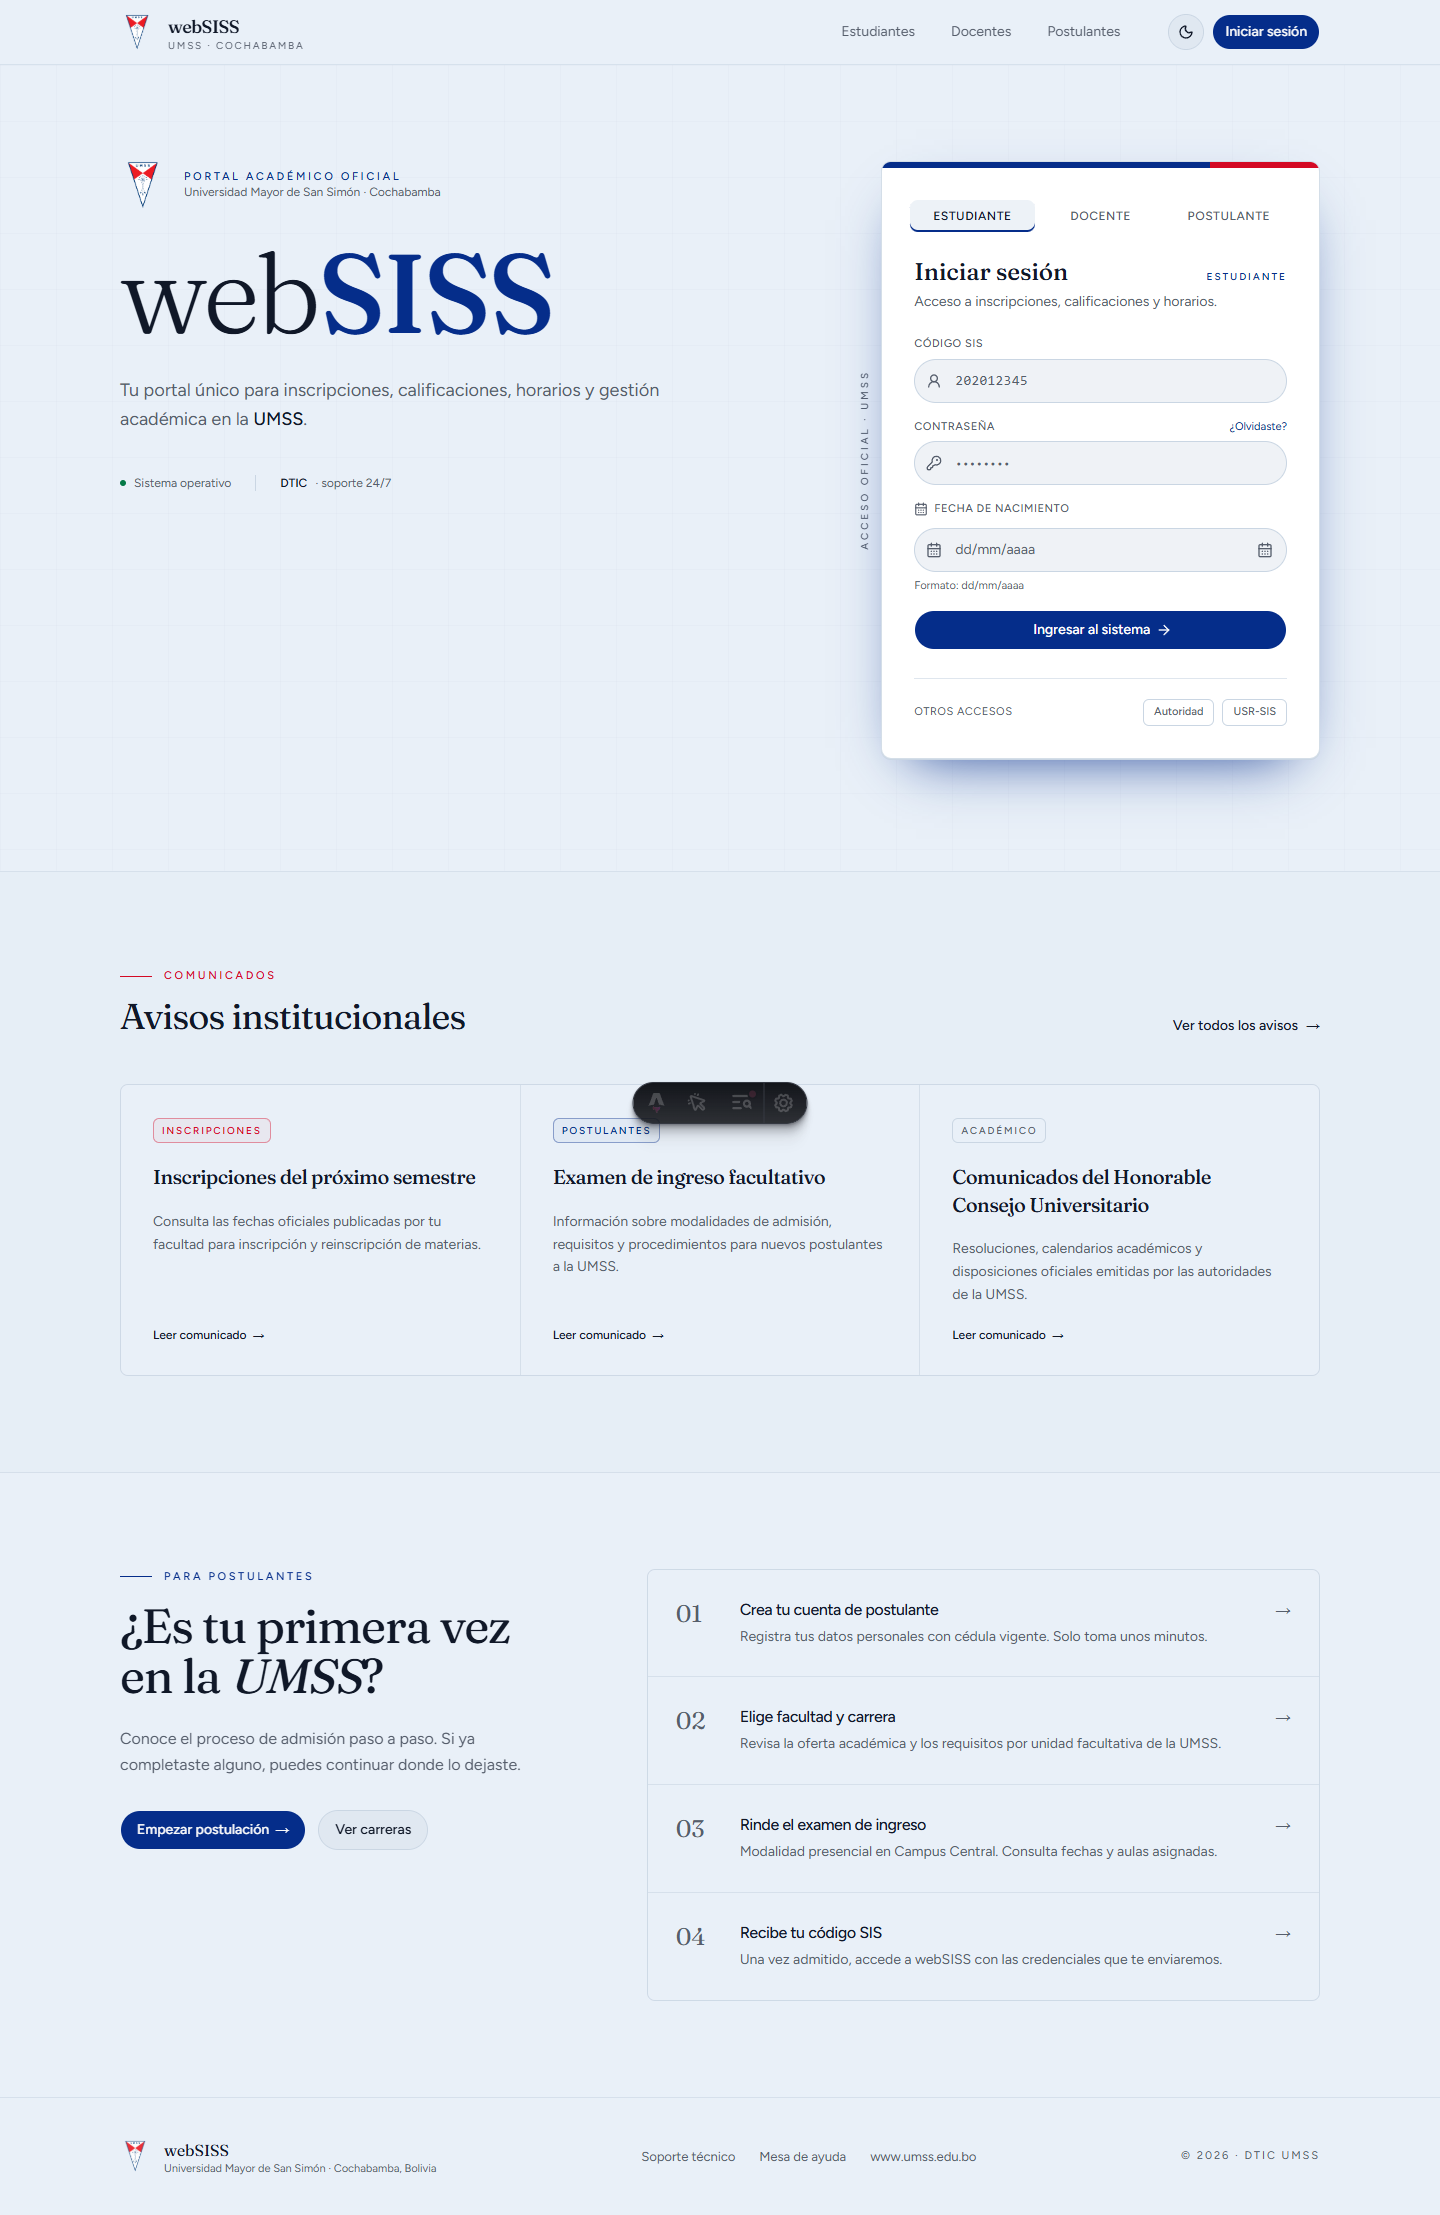
\includegraphics[width=\textwidth,height=0.72\textheight,keepaspectratio]{images/prototipo/01-login.png}
  \caption{Inicio de sesion directo para estudiantes, sin pantalla de bienvenida intermedia ni CAPTCHA visual.}
\end{figure}

\begin{figure}[H]
  \centering
  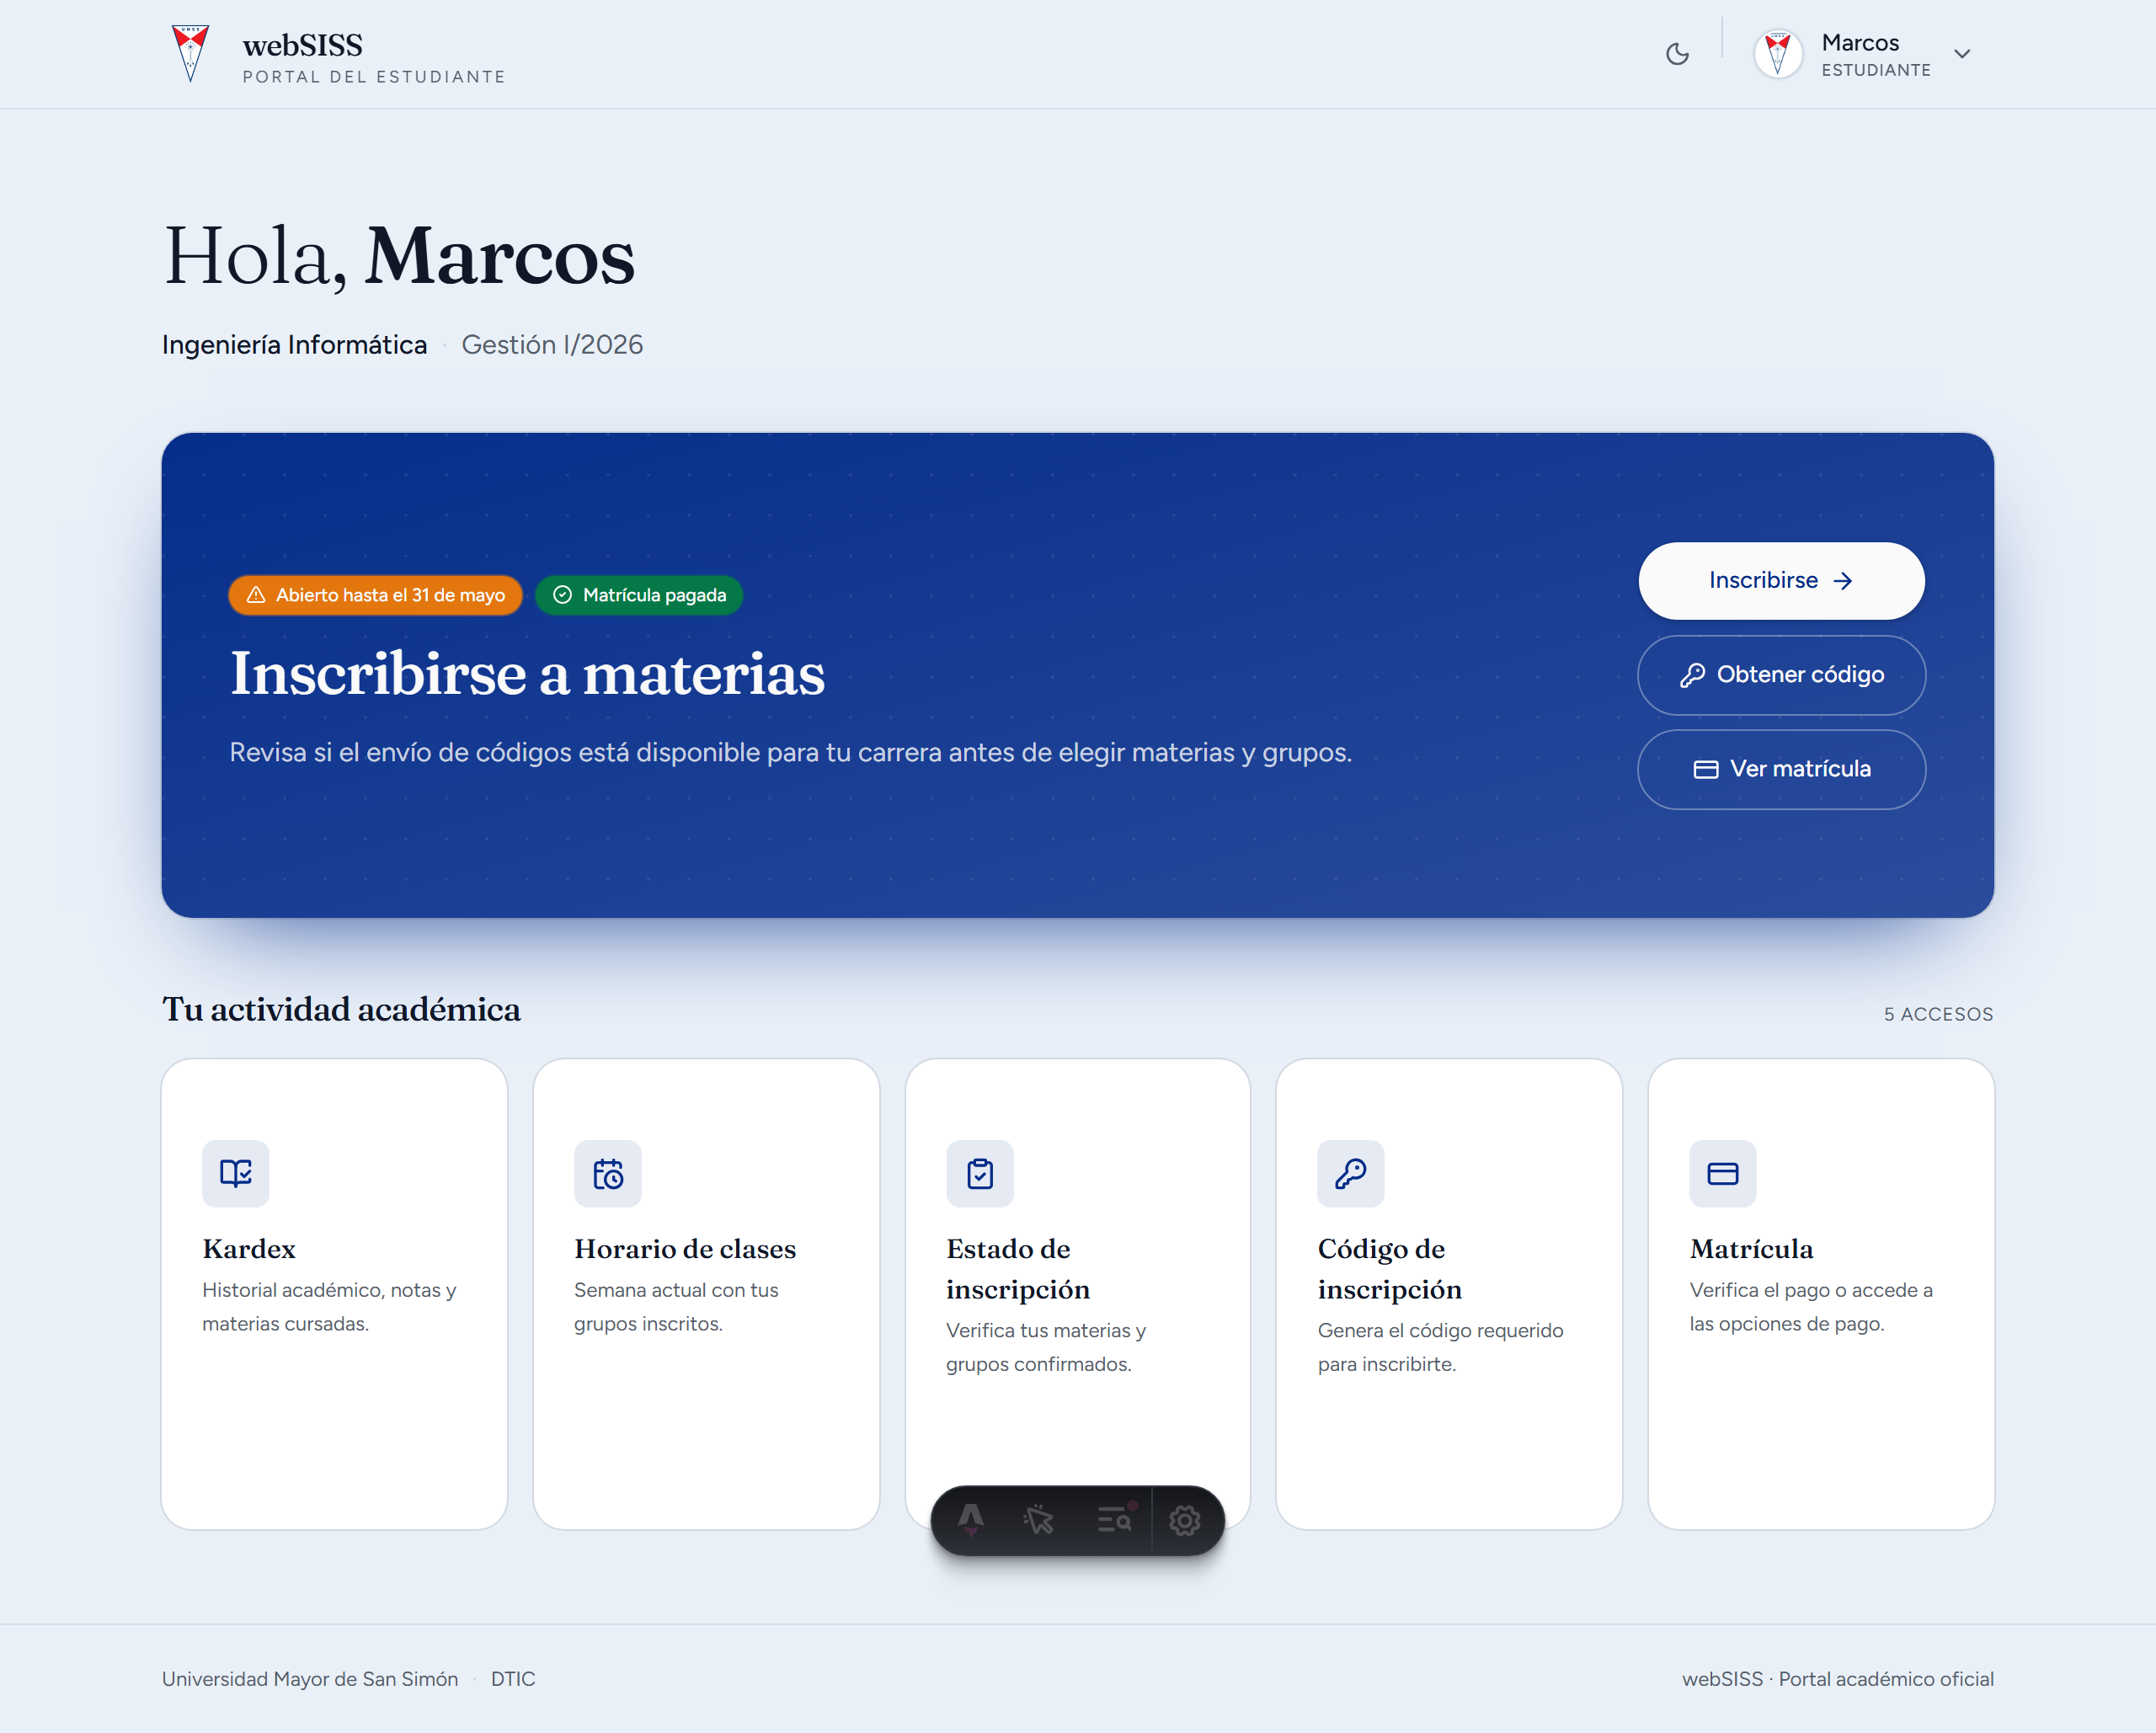
\includegraphics[width=\textwidth,height=0.72\textheight,keepaspectratio]{images/prototipo/02-panel.png}
  \caption{Panel principal con acciones priorizadas, estado de matricula y accesos academicos compactos.}
\end{figure}

\begin{figure}[H]
  \centering
  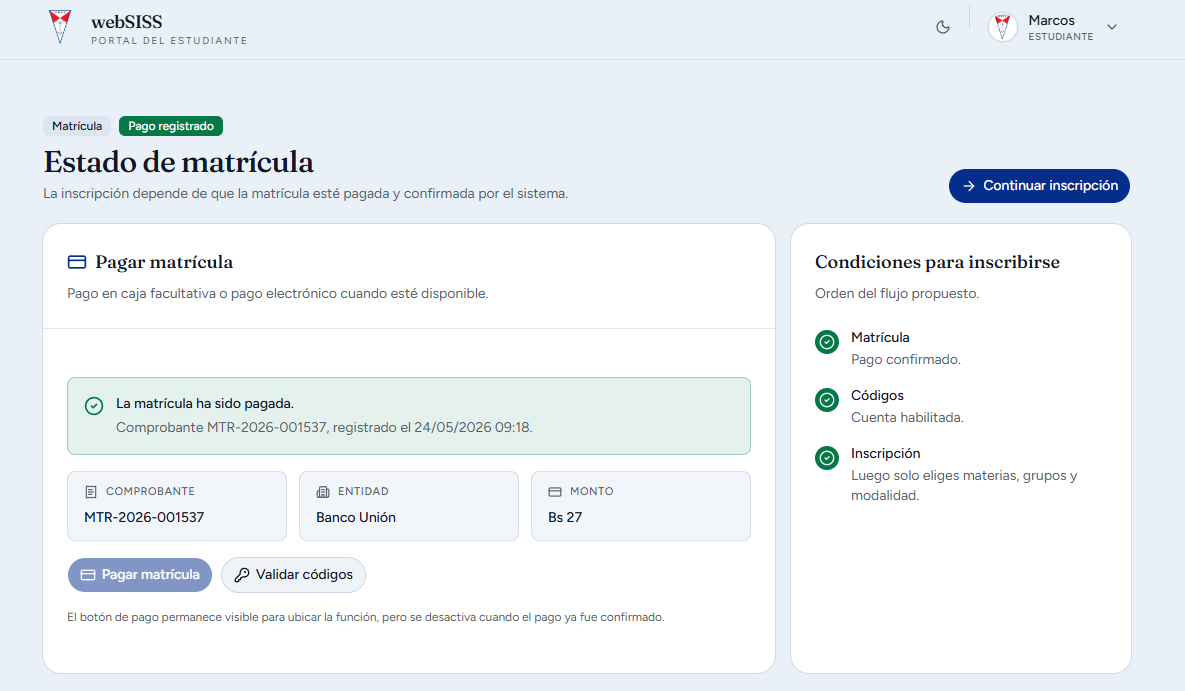
\includegraphics[width=\textwidth,height=0.72\textheight,keepaspectratio]{images/prototipo/03-matricula.png}
  \caption{Estado de matricula con comprobante, entidad de pago y boton de pago contextual.}
\end{figure}

\begin{figure}[H]
  \centering
  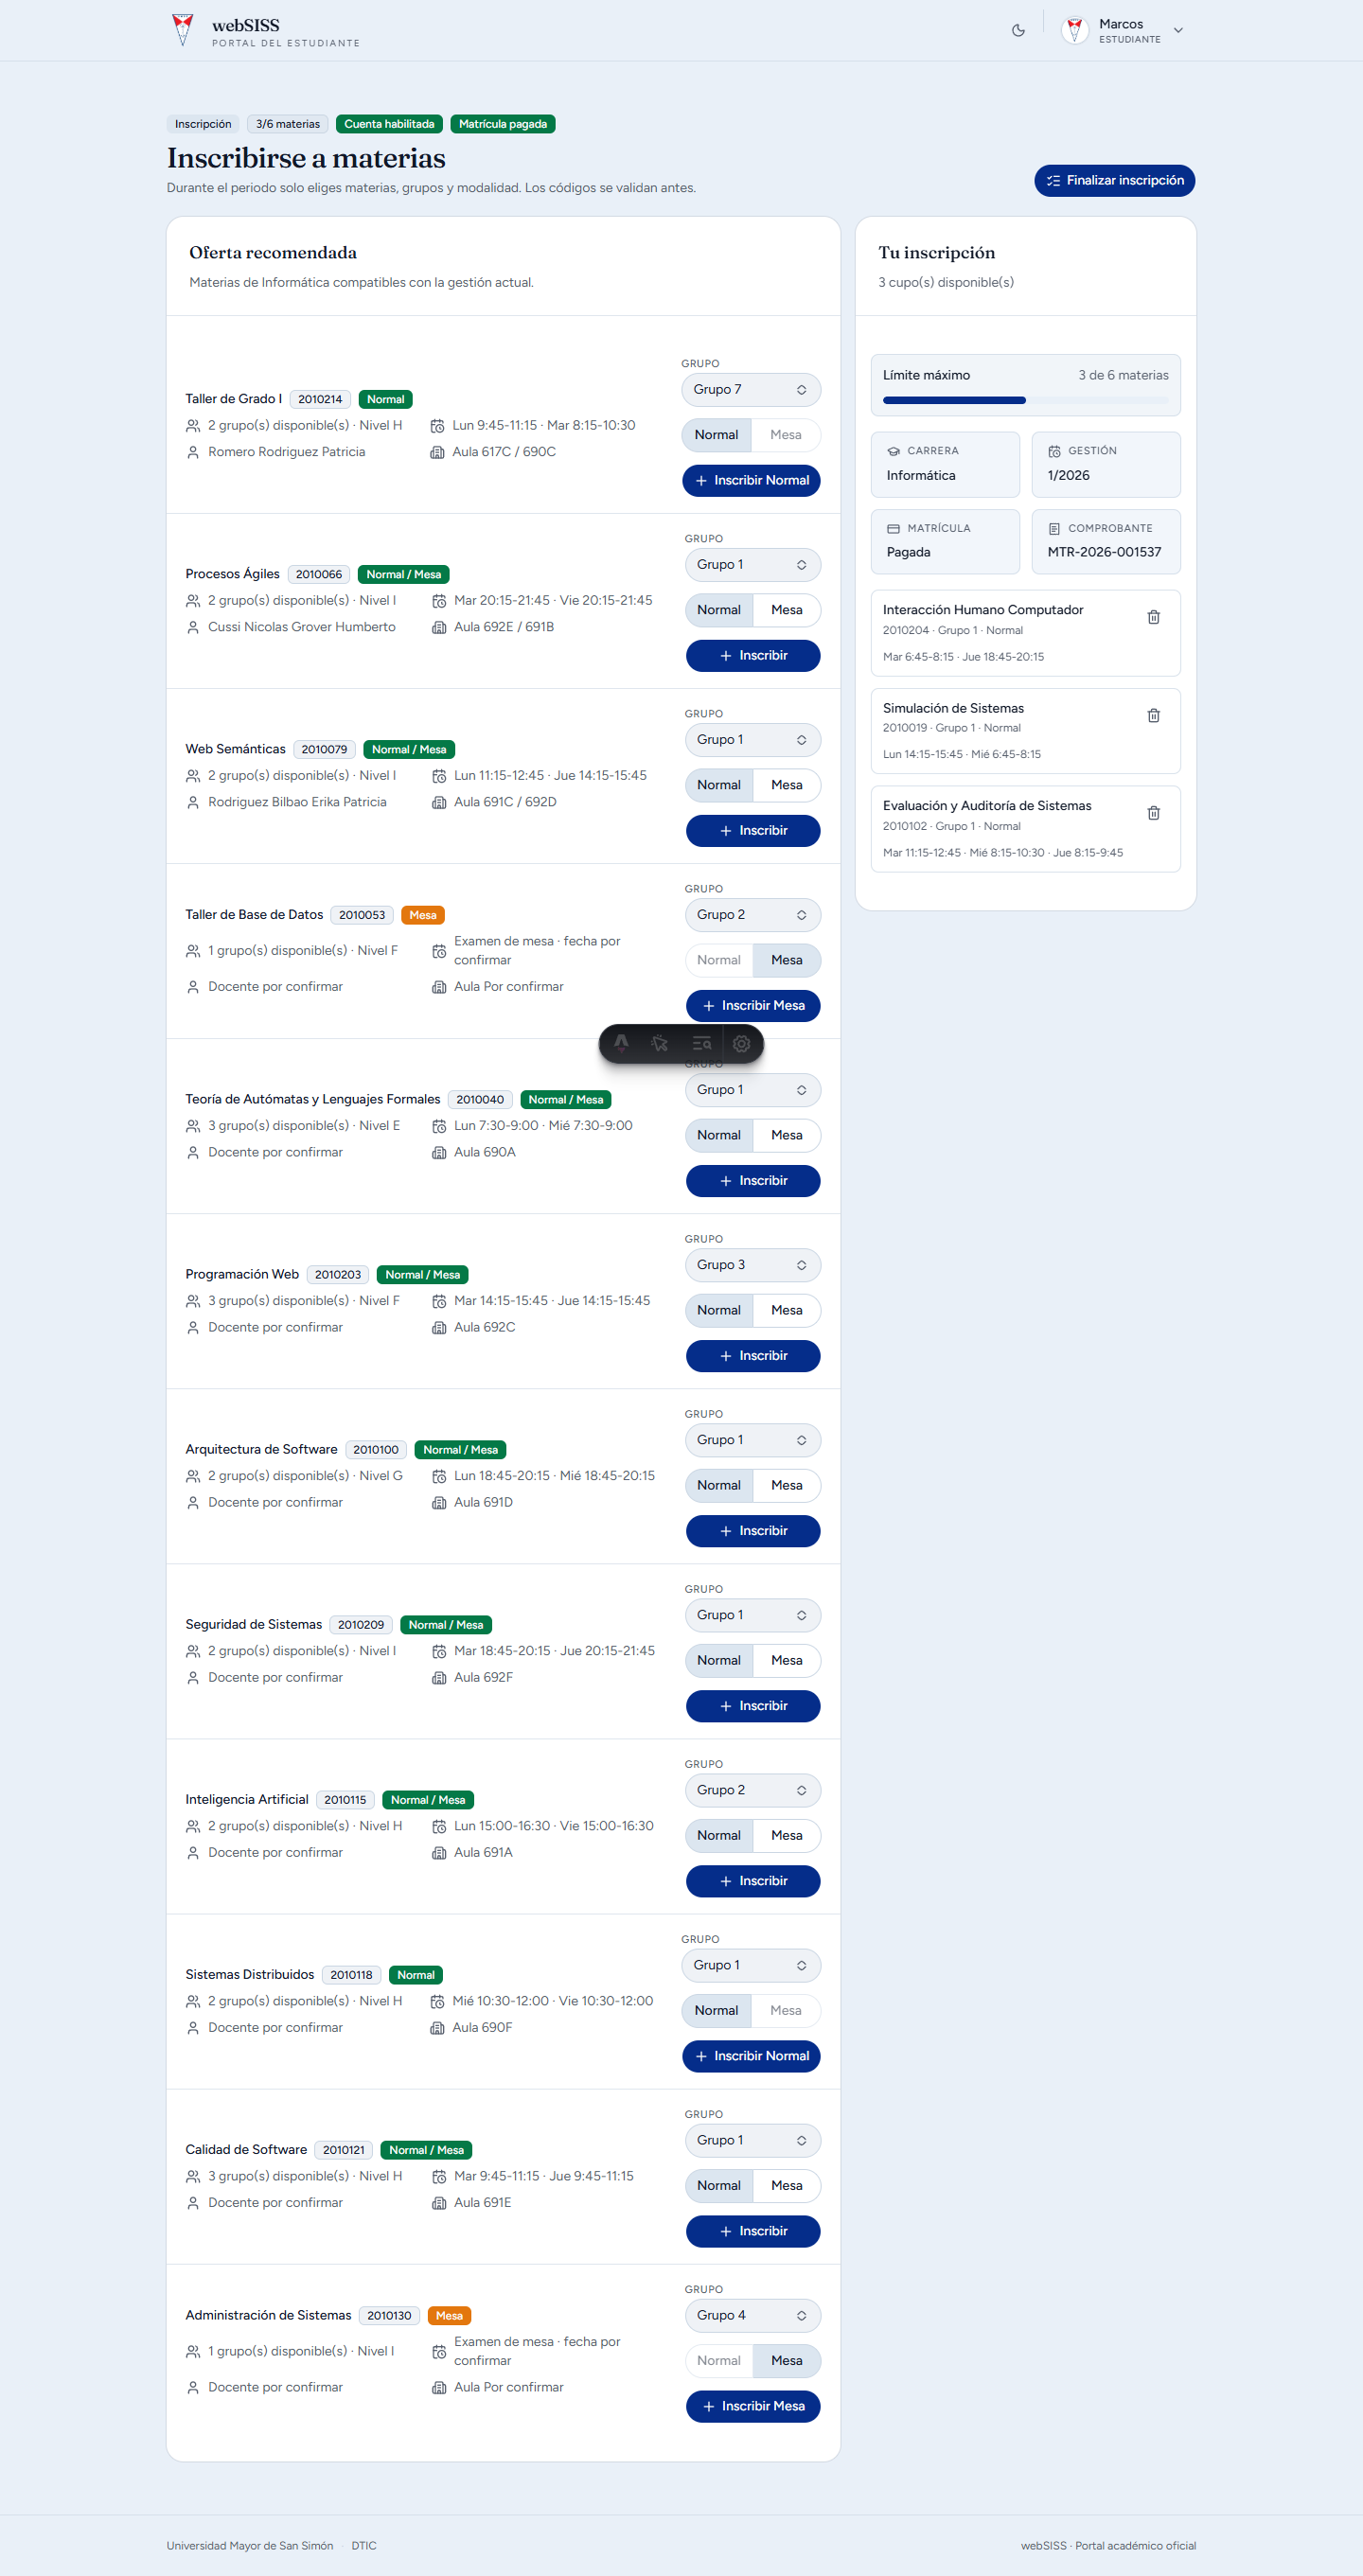
\includegraphics[width=\textwidth,height=0.72\textheight,keepaspectratio]{images/prototipo/05-inscripcion.png}
  \caption{Modulo de inscripcion con limite visible, seleccion de grupo, modalidad y resumen lateral.}
\end{figure}

\begin{figure}[H]
  \centering
  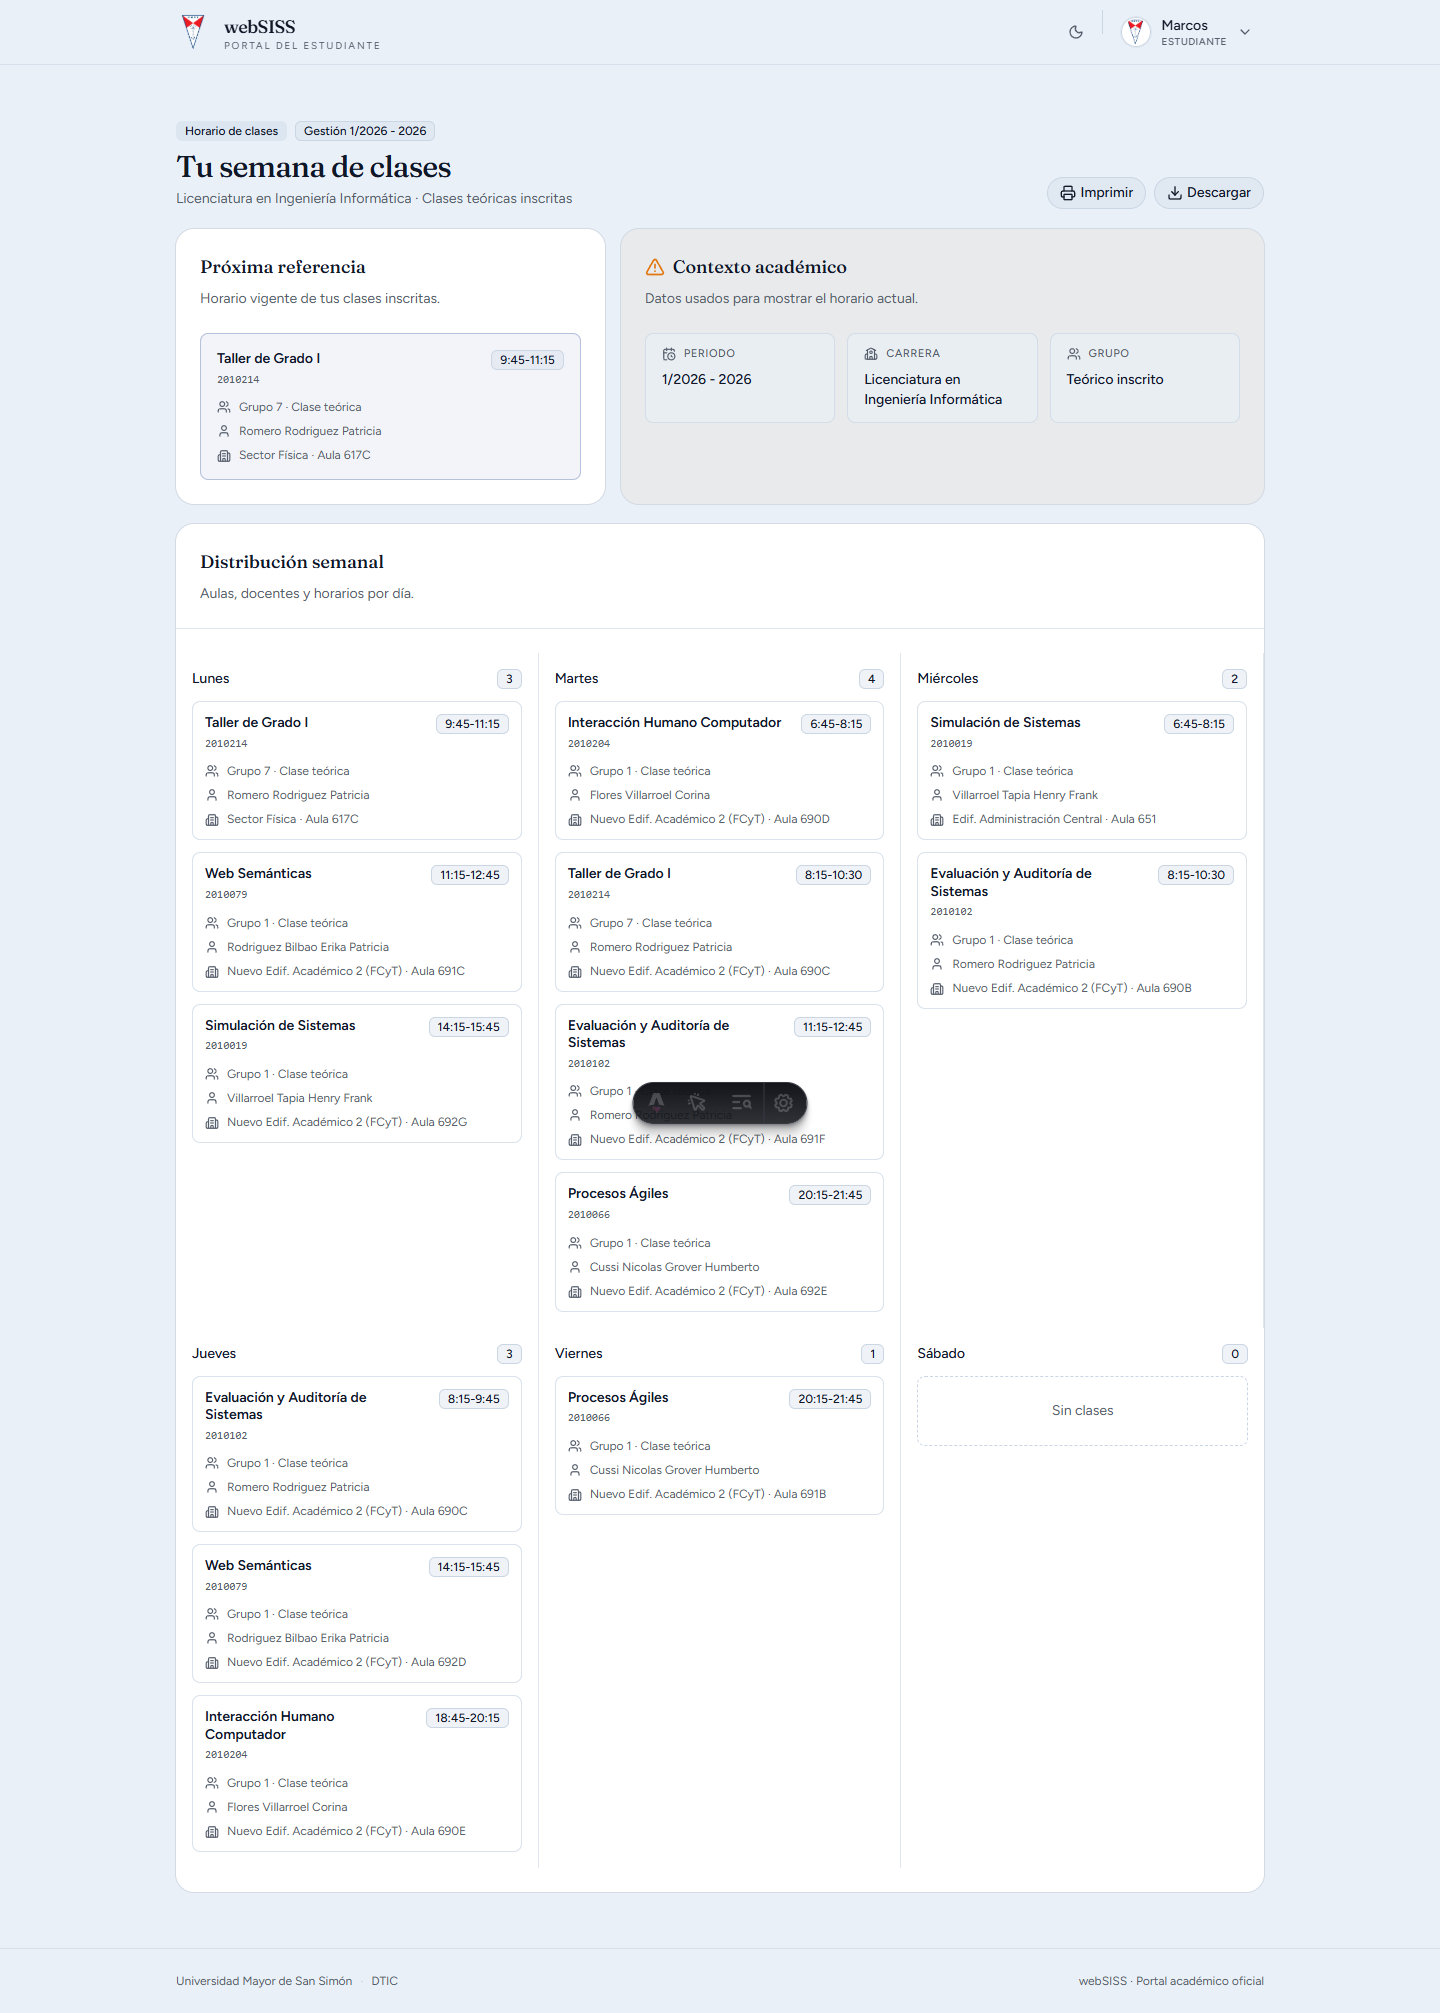
\includegraphics[width=\textwidth,height=0.72\textheight,keepaspectratio]{images/prototipo/07-horario.png}
  \caption{Horario vigente mostrado directamente, sin filtros de gestiones irrelevantes.}
\end{figure}

\begin{figure}[H]
  \centering
  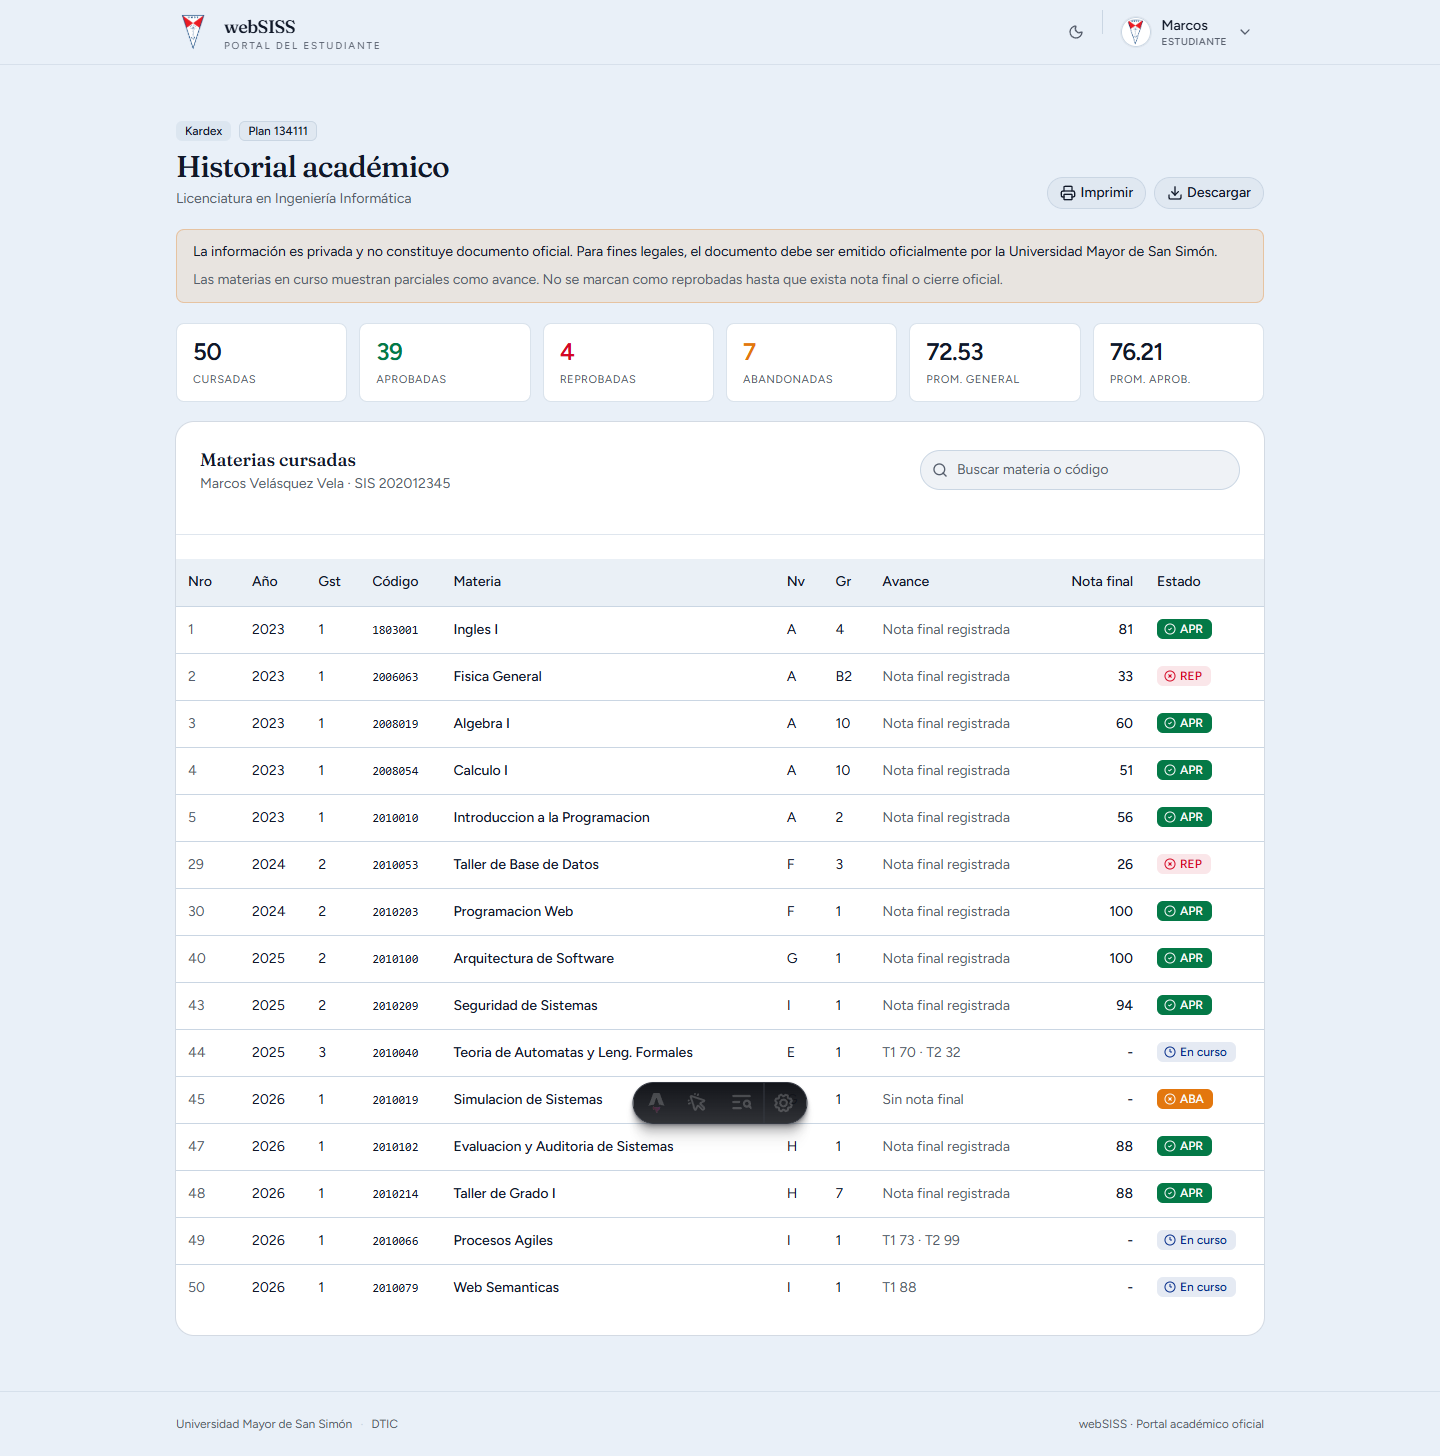
\includegraphics[width=\textwidth,height=0.72\textheight,keepaspectratio]{images/prototipo/08-kardex.png}
  \caption{Kardex reorganizado con materias cerradas y materias en curso diferenciadas.}
\end{figure}

\subsection{Validacion de la propuesta con usuarios}

Las decisiones de estructura y los wireframes no se sostienen unicamente en principios teoricos: fueron contrastadas con estudiantes reales de la UMSS mediante dos tecnicas complementarias. El \textit{card sorting} se utilizo para verificar que la arquitectura de informacion coincidiera con el modelo mental del estudiante (necesidad N5), mientras que las pruebas de usabilidad sobre los wireframes permitieron comprobar que los flujos propuestos pudieran completarse sin asistencia. Ambas tecnicas se aplicaron sobre los mismos perfiles observados en la investigacion: estudiantes ingresantes y estudiantes avanzados de la facultad.

\subsubsection*{Card sorting: validacion de la arquitectura de informacion}

Se aplico un \textit{card sorting hibrido} con 8 estudiantes (4 ingresantes y 4 avanzados). A cada participante se le entregaron 10 tarjetas, cada una con una funcion del sistema redactada en lenguaje del estudiante: \textit{Pagar matricula}, \textit{Ver comprobante de matricula}, \textit{Validar codigos}, \textit{Inscribirse a materias}, \textit{Estado de inscripcion}, \textit{Horario de clases}, \textit{Kardex}, \textit{Datos personales}, \textit{Cambiar contraseña} y \textit{Cerrar sesion}. Se les pidio agrupar las tarjetas segun como ellos esperarian encontrarlas y nombrar cada grupo con sus propias palabras.

\begin{itemize}
  \item \textbf{Objetivo:} verificar si la agrupacion espontanea de los estudiantes coincidia con la estructura propuesta en el mapa del sistema y en la subseccion de estructura del contenido.
  \item \textbf{Metodo:} card sorting hibrido (los participantes podian usar categorias sugeridas o crear las suyas), realizado de forma presencial e individual.
  \item \textbf{Registro:} se documentaron las agrupaciones, los nombres asignados a cada categoria y las dudas verbalizadas durante la actividad.
\end{itemize}

\noindent Los resultados de coincidencia entre la agrupacion de los estudiantes y la estructura propuesta se resumen en el siguiente cuadro:

\begin{table}[H]
\centering
\begin{tabular}{p{5.5cm} c p{5.0cm}}
\hline
\textbf{Tarjeta / funcion} & \textbf{Coincidencia} & \textbf{Categoria mas frecuente} \\
\hline
Pagar matricula & 8/8 & Matricula \\
Ver comprobante de matricula & 7/8 & Matricula \\
Validar codigos & 6/8 & Inscripcion / paso previo \\
Inscribirse a materias & 8/8 & Inscripcion \\
Estado de inscripcion & 6/8 & Inscripcion \\
Horario de clases & 8/8 & Informacion academica \\
Kardex & 8/8 & Informacion academica \\
Datos personales & 7/8 & Perfil \\
Cambiar contraseña & 5/8 & Perfil / seguridad \\
Cerrar sesion & 7/8 & Perfil / seguridad \\
\hline
\end{tabular}
\caption{Resultados del card sorting: coincidencia con la estructura propuesta.}
\label{tab:card-sorting}
\end{table}

\noindent Hallazgos principales del card sorting:

\begin{itemize}
  \item La mayoria de los estudiantes agrupo de forma natural \textit{Matricula}, \textit{Inscripcion}, \textit{Informacion academica} y \textit{Perfil}, coincidiendo con la estructura propuesta y confirmando la necesidad \textbf{N5} (navegacion alineada al modelo mental del estudiante).
  \item \textit{Validar codigos} genero dudas: 2 de 8 participantes no sabian si pertenecia a matricula o a inscripcion. Esto reforzo la decision de mantenerlo como un paso previo y separado, pero visible desde ambos contextos (Flujo 1), atendiendo la necesidad \textbf{N1} (guia en inscripcion).
  \item \textit{Cambiar contraseña} fue la tarjeta con mayor dispersion: algunos estudiantes la asociaban a configuracion general y no a seguridad. Por eso se conservo dentro del menu de perfil pero etiquetada explicitamente como accion de seguridad.
  \item Ningun estudiante ubico los datos personales como un bloque permanente en pantalla, lo que respalda la decision de trasladarlos al menu de perfil.
\end{itemize}

\subsubsection*{Pruebas de usabilidad sobre los wireframes}

Con los mismos perfiles de usuario se realizaron pruebas de usabilidad moderadas sobre los wireframes de baja fidelidad. A cada estudiante se le pidio completar tareas representativas mientras pensaba en voz alta. Se registro si la tarea se completaba sin ayuda, el numero de dudas relevantes y los comentarios espontaneos.

\begin{table}[H]
\centering
\begin{tabular}{p{6.5cm} c c}
\hline
\textbf{Tarea solicitada} & \textbf{Completada sin ayuda} & \textbf{Dudas relevantes} \\
\hline
Iniciar sesion sin pantalla de bienvenida & 8/8 & 0 \\
Verificar si la matricula esta pagada & 8/8 & 0 \\
Encontrar donde validar los codigos & 6/8 & 2 \\
Inscribirse a tres materias con grupo y modalidad & 7/8 & 1 \\
Revisar el estado final de la inscripcion & 8/8 & 0 \\
Consultar el horario vigente & 8/8 & 0 \\
Distinguir materias en curso de finalizadas en el Kardex & 7/8 & 1 \\
Cambiar la contraseña & 6/8 & 2 \\
\hline
\end{tabular}
\caption{Resultados de las pruebas de usabilidad sobre los wireframes.}
\label{tab:pruebas-wireframes}
\end{table}

\noindent Hallazgos principales de las pruebas de wireframes:

\begin{itemize}
  \item Las tareas con estado explicito (matricula, horario, estado de inscripcion) se completaron sin dificultad, validando la necesidad \textbf{N2} (confirmacion clara de las acciones).
  \item El acceso a \textit{Validar codigos} fue la tarea con mas dudas: algunos estudiantes lo buscaron primero dentro de inscripcion. Se ajusto el wireframe del panel para dar a este acceso mayor visibilidad junto a la accion principal, en linea con la necesidad \textbf{N6} (acceso rapido a tareas frecuentes).
  \item En el Kardex, 1 de 8 estudiantes no diferencio de inmediato la materia en curso; el contraste visual entre fila cerrada y fila en curso se reforzo en consecuencia, evitando que una materia sin nota final se interprete como reprobada.
  \item Los participantes que probaron los wireframes en una vista reducida confirmaron que los accesos compactos y la separacion por pantallas facilitaban la lectura en movil, en linea con la necesidad \textbf{N4} (compatibilidad movil).
\end{itemize}

\subsubsection*{Sintesis de la validacion}

En conjunto, el card sorting confirmo que la estructura propuesta coincide en gran medida con el modelo mental del estudiante, mientras que las pruebas de usabilidad demostraron que los flujos principales pueden completarse sin asistencia. Los puntos de friccion detectados (validacion de codigos y cambio de contraseña) no invalidaron la propuesta, sino que permitieron ajustar la visibilidad y el etiquetado de esos accesos antes de avanzar al prototipo. De esta forma, las decisiones de diseño quedan respaldadas no solo por principios de usabilidad, sino por evidencia obtenida directamente de los usuarios.

\subsection{Justificacion del rediseño}

\subsubsection*{Justificacion basada en usabilidad}

La propuesta responde a los principales problemas detectados heuristicamente en WebSIS y los traduce en decisiones concretas de interfaz. No se trata solo de cambiar la apariencia, sino de reducir pasos innecesarios, hacer visibles los estados criticos y usar un lenguaje cercano al estudiante de la UMSS.

\begin{itemize}
  \item \textbf{Visibilidad del estado del sistema:} el sistema anterior obligaba al estudiante a inferir si podia inscribirse, si la matricula estaba pagada o si los codigos ya estaban habilitados. Por eso se incorporan estados explicitos como \textit{matricula pagada}, \textit{cuenta habilitada}, \textit{validacion pendiente}, \textit{materia en curso} e \textit{inscripcion finalizada}.
  \item \textbf{Correspondencia con el mundo real:} se evita terminologia tecnica o ajena al contexto local y se usa \textit{Panel del estudiante}. Las secciones se nombran segun tareas reconocibles: pagar matricula, validar codigos, inscribirse, ver horario, consultar Kardex y cambiar contraseña.
  \item \textbf{Control y libertad del usuario:} en la inscripcion el estudiante puede revisar materias, elegir grupo, seleccionar modalidad normal o mesa, retirar materias y confirmar solo cuando el resumen sea correcto. Esto evita que una accion parcial se perciba como irreversible.
  \item \textbf{Prevencion de errores:} se separa la validacion de codigos del momento critico de inscripcion, se deshabilita el boton de pagar matricula cuando el pago ya fue confirmado y se evita marcar como reprobada una materia sin nota final.
  \item \textbf{Reconocimiento antes que recuerdo:} el panel principal concentra accesos directos a tareas frecuentes, evitando que el estudiante tenga que recordar rutas, pasos o menus internos del sistema.
  \item \textbf{Eficiencia de uso:} horario, Kardex y estado de inscripcion se muestran directamente con la gestion vigente, sin pedir años, periodos o planes que no aportan valor para la tarea inmediata.
\end{itemize}

\subsubsection*{Justificacion basada en leyes de la Gestalt}

La organizacion visual del prototipo se apoya en principios de percepcion que facilitan lectura, orientacion y toma de decisiones:

\begin{itemize}
  \item \textbf{Proximidad:} los datos que forman una misma decision se presentan juntos. En inscripcion, materia, grupo, modalidad, docente y horario aparecen dentro de una misma unidad; en matricula, comprobante, entidad y fecha se agrupan en el mismo bloque.
  \item \textbf{Similitud:} los accesos directos usan la misma estructura visual para que el estudiante reconozca que son acciones equivalentes. Esto reduce exploracion innecesaria y mejora la lectura en movil.
  \item \textbf{Jerarquia figura-fondo:} las acciones prioritarias, como \textit{Inscribirse}, \textit{Pagar matricula} o \textit{Validar codigos}, se distinguen de informacion secundaria. Asi el siguiente paso no queda oculto entre avisos o paneles laterales.
  \item \textbf{Continuidad:} los flujos se ordenan de forma secuencial y comprensible: matricula, validacion de codigos, seleccion de materias y estado final. Esta progresion coincide con el orden real del proceso academico.
  \item \textbf{Region comun:} las tarjetas, tablas y paneles delimitan contextos de informacion. Kardex, horario, inscripcion y seguridad no compiten en una sola pantalla, sino que se separan por ruta y por objetivo.
\end{itemize}

\subsubsection*{Justificacion basada en carga cognitiva}

El rediseño busca disminuir la carga cognitiva extrinseca que actualmente impone WebSIS, especialmente durante tareas de alta presion como la inscripcion. La interfaz anterior obligaba a interpretar informacion dispersa, repetir codigos, revisar pantallas intermedias y decidir entre opciones que no siempre correspondian al estudiante.

\begin{itemize}
  \item se elimina la pantalla de bienvenida porque no aporta a la tarea principal de ingreso;
  \item se simplifica el inicio de sesion al usar una fecha escrita con formato visible y eliminar el CAPTCHA visual;
  \item se hace visible el estado de matricula para que el estudiante no tenga que inferir si puede inscribirse;
  \item se reduce la repeticion innecesaria de codigos durante inscripcion mediante una habilitacion previa;
  \item se eliminan filtros irrelevantes en horario y Kardex, como gestiones o periodos que no corresponden al estudiante;
  \item se evita que una materia en curso sea interpretada como reprobada cuando solo existen notas parciales;
  \item se divide el proceso en estados comprensibles y con retroalimentacion inmediata;
  \item se adapta la densidad de informacion a movil mediante accesos compactos, resumen progresivo y separacion de pantallas.
\end{itemize}

En conjunto, estas decisiones permiten que el estudiante concentre su esfuerzo en la tarea academica real y no en descifrar como funciona la interfaz. El rediseño mejora la utilidad percibida, disminuye ansiedad en periodos criticos y hace que el sistema se comporte de acuerdo con el modelo mental del estudiante.
